Voici une présentation de l'interface et ses fonctionnalités.

\subsection{Interface}
Voici comment se présente notre interface : 
\begin{figure}[!h]
    \centering
    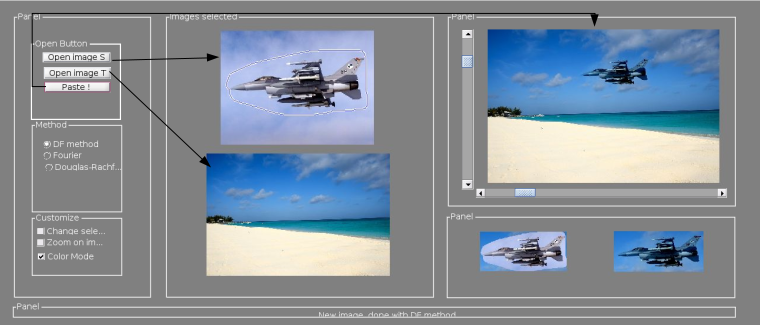
\includegraphics[scale = 0.3]{Images/interface.png}
    \caption{Interface 1.0}
\end{figure}{}
Elle est découpée en "blocs". Le premier bloc appelé "Open Button", se situe en haut à gauche, il permet l'ouverture d'images.En cliquant sur "Open Image S", une boite de dialogue s'ouvre et permet de charger une image, présente dans l'ordinateur. De même en cliquant sur le bouton T. Une fois ces images chargées elle s'affiche dans le bloc numéro 2 appelé "Images displayed". L'image la plus haute dans ce bloc correspond à l'image S, tandis que l'image si situant en bas affiche l'image T.
Il y a aussi un bouton "Save" permettant d'enregistrer l'image obtenue.\\ Une fois les images affichées, il faut sélectionner la région dite "à coller" dans l'image S,  et la région où va se faire le collage dans l'image T.\\

\paragraph{Choix des méthodes}
Dans cette interface il est possible de sélectionner la méthode à utiliser. Le choix se porte sur 3 algorithmes : 
\begin{itemize}
    \item Les différences finies
    \item Fourier 
    \item Douglas-Rachford
\end{itemize}{}
IL suffit de sélectionner la méthode pour l'appliquer.
En cliquant sur le bouton "Paste !", présent dans le bloc numéro 1, la nouvelle image est calculée et s'affiche dans le bloc "Main Result" situé en haut à droite. 
\paragraph{Les options}
D'autres options s'offrent à vous dans cette interface. Il est possible d'effectuer l'amélioration vue plus haut, en la sélectionnant, case : "Change selection". Il est aussi possible de zoomer sur les différentes images, à l'aide de la case zoom. Enfin il est possible de travailler sur des images en couleur, en cochant la case adéquate. Toutes ces options se trouvent dans e bloc :Customizer.
\paragraph{Sliders}
Des sliders sont situés de part et d'autres de l'image finale, dans le bloc "main result". En activant ces sliders, il est donc possible de bouger la sélection à l'intérieur de l'image. Ainsi, l'image finale est recalculée, et l'image à coller, sera collée à la position indiquée par les sliders.
\paragraph{bloc Results}
Le dernier bloc est un bloc d'affichage, il affiche une fois créée l'image obtenue par l'algorithme sélectionné, dans le bloc correspondant, cela permet une comparaison rapide.
\subsection{Organisation du code}
Nous avons organisé le code sous forme de classes. Le projet contient 4 classes principales, la classe, Fourier, la classe DFinies, la classe Douglas et enfin la classe  Mask. Notre projet contient aussi deux fonctions, la fonctions copier/coller et la fonction du gradient conjugué.

%%%%%%%%%%%%%%%%%%%%%%%%%%%%%%%%%%%%%%%%%%%%%%%%%%%

\begin{figure}
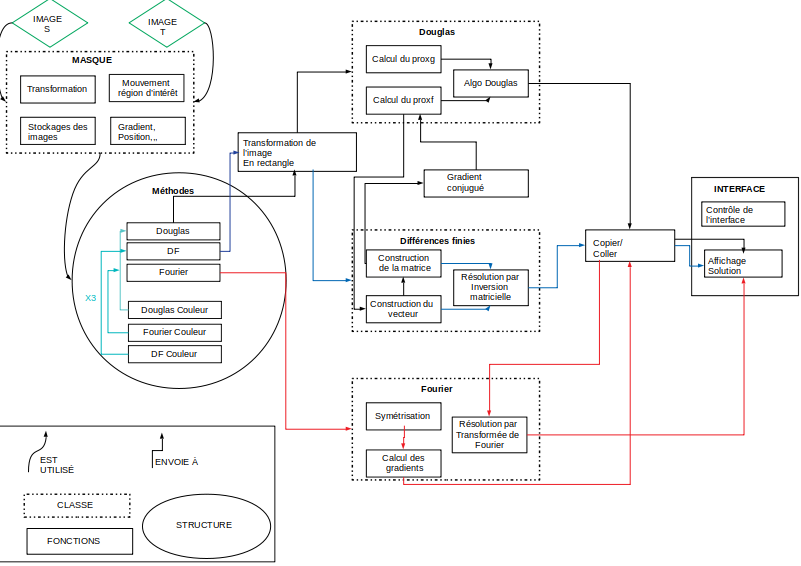
\includegraphics[scale=0.65]{Images/code/schema.png}
\caption{Structure et interactions du code}
\end{figure}
\newpage

\paragraph{Explication du schéma}
Le code est organisé en différentes classes (4).
\paragraph{Douglas}
Cet algorithme étant plutôt long (en terme de temps), nous ne travaillerons pas sur l'image entière mais sur le plus petit rectangle autour de la sélection.En d'autre terme nous collerons l'image S sur une sous-image de T, que nous réinsérerons par la suite au bon endroit dans T. Afin de résoudre le problème à l'aide de l'algorithme de Douglas, nous avons crée une classe du même nom.  A l'intérieur de celle-ci nous calculons les opérateurs proximaux nécessaires. Avec une particularité, l'opérateur proximal de la norme, nécessite la construction d'une matrice. Afin d'éviter les doublons nous utilisons donc la classe FDSystem, pour calculer cette matrice, et le vecteur associé. Puis nous inversons le système à l'aide de l'algorithme du gradient conjugué. 
\paragraph{Différences finies}
Pour résoudre le problème avec les différences finies, la classe DFSystem, nous permet de calculer la matrice A, le vecteur b et enfin d'inverser le système pour trouver la solution. De la même manière que pour Douglas, nous ne travaillons pas sur l'image entière mais sur une sous-image que nous recollons au bon endroit à la fin.
\paragraph{Fourier}
Dans la classe Fourier nous symétrisons les images, puis calculons les gradients de celles-ci. Les images représentant les gradients sont par la suite fusionnées avant d'être envoyé à la fonction de résolution de la classe Fourier. 
\paragraph{Mask}
La classe Mask, permet le traitement d'images et de masque, elle est mise à jour pendant tout le programme. C'est notamment elle qui permet le découpage d'image, la fusion de deux images, le redimensionnement des masques si besoin. 
\paragraph{La fonction gradient conjugué}
Elle permet de trouver la solution au système Ax=b de manière plus rapide qu'une inversion dans matlab.
\paragraph{La fonction copier coller} 
Elle écrase certains pixels d'une image par les pixels d'une autre.